
\section{Laser stand for the MAPMT characterization}
The large number of the channels in the RICH detector  poses challenging problem for the MAPMT testing and calibration.
RICH consists of 391 MAPMTs resulting in total number of channels equal to 25024. So in order to test them efficiently within a reasonable timeframe the fully automated test stand was build to evaluate 6 MAPMTs at once, as shown on Fig.~\ref{fig:MAPMTtest}.

\begin{figure}[hbt]
	\centering
	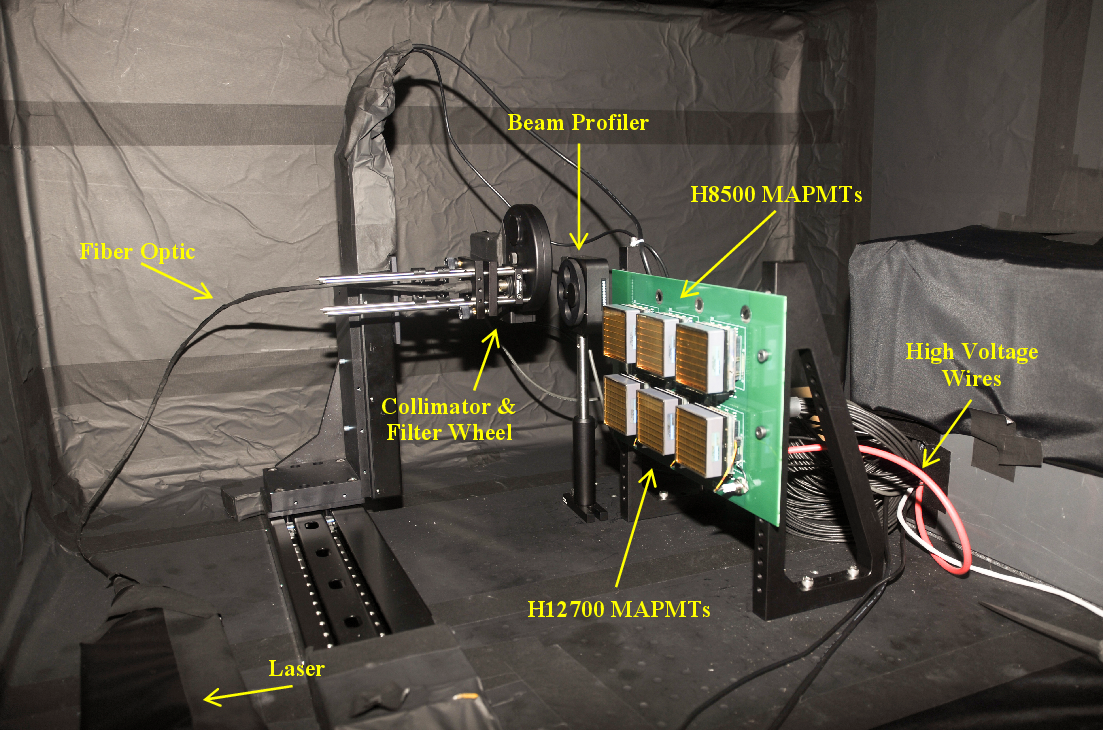
\includegraphics[width=0.9\linewidth]{blackbox.png}
	\caption{Inner view of the laser stand.}
	\label{fig:MAPMTtest}
\end{figure}

The test stand consists of picosecond diode  laser PiL047X with 470 nm wavelength, 2 long travel motorized stands to drive laser fiber in two dimensional space for individual pixel illumination, the motorized wheel with neutral density filter system, 2 adapter boards for MAPMT with JLab designed front-end electronics boards \cite{}{Contalbrigo:2020}.
The laser light is directed through the fiber and attenuated to the single photon level using the neutral density filters to mimic the conditions of the RICH detector.
The motors were remotely controlled to move the focused laser beam across (see Fig.~\ref{fig:beamopt1}) the entire surface of the MAPMT entrance window and illuminate one by one of all its 64 pixels individually.
Another option is to illuminate the whole surface of MAPMT photocathode at once using the Engineered Diffuser to produce square pattern with non-Gaussian intensity distribution (see Fig.~\ref{fig:beamopt2}). 

All laser stand equipment is sitting in the black box with non-reflective black material on the optical table. The laser interlock safety box automatically switch off laser, as well as front-end low voltage  electronics and MAPMT high voltage to prevent the possible photomultiplier damage or laser light human illumination in case if somebody will try to open the front door of the black box during the measurements.

\begin{figure}[bt]
	\centering
	\begin{subfigure}[b]{0.628\linewidth}
		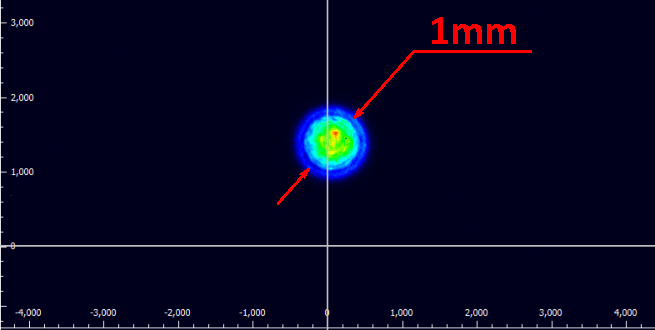
\includegraphics[width=\textwidth]{beamspot.pdf}
		\caption{Focused laser beam with the dimension much less than the  MAPMT pixel size.}
		\label{fig:beamopt1}
	\end{subfigure}
	\begin{subfigure}[b]{0.354\linewidth}
		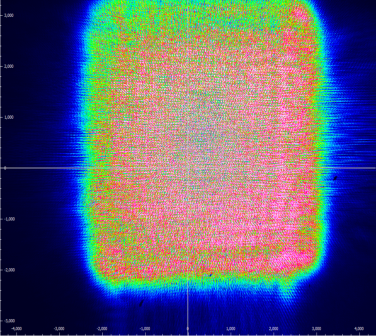
\includegraphics[width=\textwidth]{beamsquare.pdf}
		\caption{Square pattern illuminated all MAPMT surface.}
		\label{fig:beamopt2}
	\end{subfigure}
	\caption{The laser light output options.}
\end{figure}

This configuration brings routine workload to minimum allowing the evaluation of 6 MAPMTs (equivalent to 328 conventional PMTs!) at 4 different high voltages and 6 different light intensities within 6 hours with less than 15 minutes of human intervention needed to load the MAPMTs to the front-end boards.

\begin{figure}[b]
	\centering
	\begin{subfigure}{0.3\linewidth}
		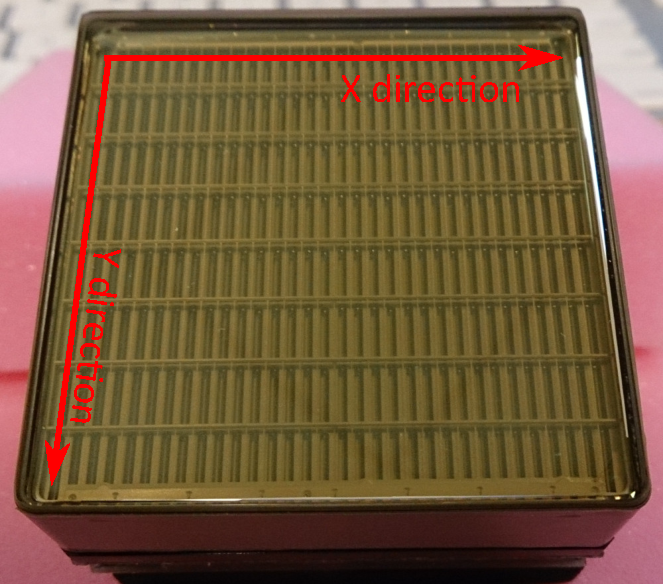
\includegraphics[width=\textwidth]{surfaceuniform1.pdf}
		\caption{MAPMT with visible internal structure of metal channel dynodes and focusing mesh.}
		\label{fig:surfaceuniform1}
	\end{subfigure}
	\quad
	\begin{subfigure}{0.3\linewidth}
		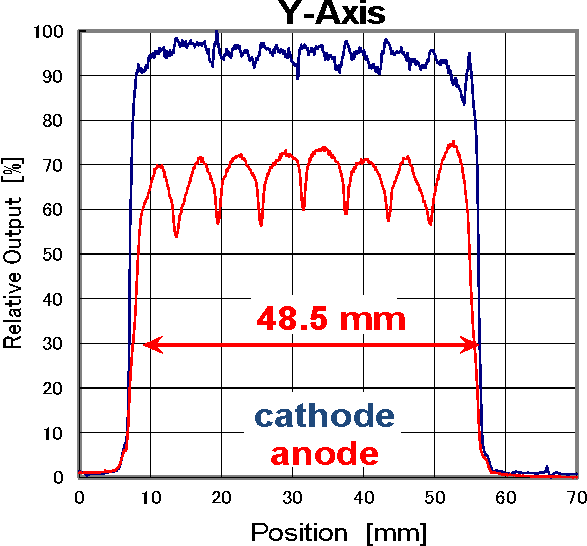
\includegraphics[width=\textwidth]{surfaceuniform3.pdf}
		\caption{The response along the X axis; the signal drops in the deadspace between the pixels.}
		\label{fig:surfaceuniform2}
	\end{subfigure}
	\quad
	\begin{subfigure}{0.3\linewidth}
		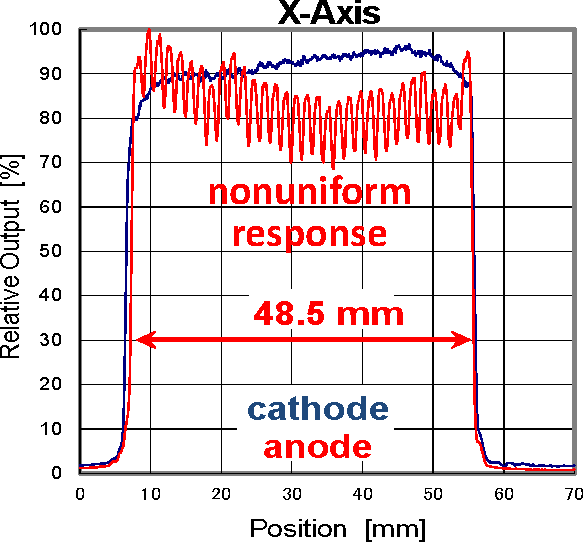
\includegraphics[width=\textwidth]{surfaceuniform2.pdf}
		\caption{The response along the Y axis: multiple segmentations within the pixels.}
		\label{fig:surfaceuniform3}
	\end{subfigure}
	\caption{The response uniformity of MAPMT.}
	\label{fig:surfaceuniform}
\end{figure}


Before starting the systematic study of the MAPMT responses, a finer two dimensional scan of several pixels was performed in order to verify the uniformity of the response across pixel's surfaces, as shown on Fig.~\ref{fig:surfaceuniform}.
The horizontal and vertical axes denote laser beam position during the scan.
Along the both directions there are obvious drops in efficiency when the laser strikes the space between the pixels.
The drops are relatively narrow so the dead-space is very small as expected from the Hamamatsu specifications.
Additionally, a vertical efficiency variation is visible across the pixel in horizontal scan.
These inhomogeneities are correlated with the vertical walls separating dynode chains, owing to the constructional features of the MAPMT. The discontinuity in dynode structure is visible  on Fig.~\ref{fig:surfaceuniform1}.
The separate response maps for photocathode shows relatively uniform signal without efficiency drops, confirming that the variation arises from the dynode system.
